\documentclass[a4paper,man,12pt,apacite,floatsintext,draftfirst]{apa6} % man => jou
\usepackage[english]{babel}
\usepackage[utf8]{inputenc}
\usepackage{mathtools}
\usepackage{url}
\usepackage{tikz}
\usepackage{listings}
\usepackage{framed}
\usepackage{etoolbox}
\usepackage{float}
\usepackage{todonotes}
\usepackage{minted}

\usemintedstyle{autumn}

\floatstyle{boxed}
\restylefloat{figure}

\BeforeBeginEnvironment{verbatim}{\def\baselinestretch{1}\noindent}

\tikzset{
  treenode/.style = {align=center, inner sep=2pt, text centered,
    font=\sffamily, minimum size=0.5cm},
  arn_c/.style = {treenode, rectangle, draw=black},
  arn_d/.style = {treenode, ellipse, draw=black}
}

\title{Random Forests: Introduction, Parts, Variants}
\shorttitle{Random Forests: Introduction, Parts, Variants}
\author{Tobias Ammann}
\authornote{Tobias Ammann\\Alte Landstrasse 39\\8802 Kilchberg\\tag@adnm.ch}
\keywords{ensemble methods, introduction, random forests}
\affiliation{Literature Study at the Workgroup for Psychological Methods,\\Evaluation and Statistics, Department of Psychology.\\Supervised by Prof. Dr. Carolin Strobl}
\note{DRAFT Version: \today}
\keywords{bagging, boosting, decision trees, ensemble methods, error estimates, fuzzy random forests, introduction, optimality criterion, out-of-bag data, overfitting, PERT, random forests, regression, rotation forests, statistics, variable importance}

\abstract{This report discusses a family of machine learning algorithms called
random forests, their structure, problems, and a number of suggested
improvements, to give the reader a general introduction, starting with the motivation,
for machine learning, and the statistical as well as historical background to machine learning and random forests. 
The aim of this work is to introduce the different parts of random forest algorithms
by giving an overview over their limitations and suggestions on overcoming these limitations.
These components are illustrated with source code snippets and comparisons between
various variants of the random forest algorithms are being made.
This report also puts forward a few ideas on how to make random forests better
and more user-friendly.}

\begin{document}
\addtocounter{page}{-1} % start page counter after title page

\thispagestyle{empty} % remove page number on title page
\maketitle

\tableofcontents

\newpage
\section{Declaration of Independence}
Hiermit versichere ich, dass ich die vorgelegte Arbeit selbständig und
ohne  unerlaubte Hilfsmittel verfasst habe.
Andere als die angegebenen Hilfsmittel habe ich nicht verwendet.
\\[3cm]

Tobias Ammann\\Datum: \today

\newpage
\section{Introduction}

\subsection{Motivation}
Psychology has come a long way as a science, with psychological research
more and more following
the \emph{scientific method}.
Research works by the assumption that if we only disprove just enough
alternative theories, we can eventually tell which theory is probably
true, despite positive proof being impossible without complete knowledge.
So, the scientific method really is nothing but the use of countless
attempts to disprove alternative theories, until only a single such theory
remains.

Since there is a large number of theories to disprove, and every
researcher likes to see the result of his work as soon as possible, a
more speedy method is usually employed, although this comes with a caveat.
The speedier method has the researcher compare his favoured theory against
the null hypothesis and show the superiority of his favoured theory.
The null hypothesis is either an alternative theory or a chance effect.
This is way more efficient than comparing the thousands of
theories that researchers have come up with, and continue to come up with.
The caveat is commonly called confirmation bias, because researchers focus
on immunising their theory instead of disproving those of others.
Therefore, the result only has significance in the experimental set-up
being tested.
On the greater scale of things, i.e. reality, the results might well be
completely bogus.
Nonetheless, most of the subjects being studied are sufficiently constant
or change predictably enough to allow researchers to generalise from the
results of an experiment to the world at large, and likely remain correct.
This likelihood depends on the size of the effects measured in the
experiment, the amount of experimental data collected,
and on the properties of the statistical methods involved.
In psychological research, where large effects are rare and
experiments often only study a handful of psychology students, who
notwithstanding research ethics are often forced to participate, it is
vital to use powerful statistical methods, because this is the only parameter
remaining for researchers to tweak in their favour.

Recently, researchers in psychology began to turn to a new breed of
statistical methods, in hope of ever better results. This new breed of
statistical methods is called \emph{machine learning}.

In this paper, I aim to introduce the reader to \emph{random forests},
which are just one family of machine learning algorithms.
I first give the reader some context to random forests, in hope that a
broader view will help developing an intuition for random forests.

In the next sections I introduce the reader to machine learning,
the differences between the traditional statistical approach and the
machine learning approach, and random forests in particular.
I then delve into some improvements to random forests that have been
suggested in the literature, call for a new random forest variant, and finish
with a few words on the method of writing this paper, and a discussion.

\subsection{Machine Learning}
In order to understand random forests, it might be useful to set
the stage by briefly discussing machine learning in general.
Machine Learning is both a part of predictive statistics and the
artificial intelligence branch of computer science.

\emph{Predictive statistics} is the sub-field of statistics that is
concerned with making predictions based on past observations.
It's probably most widely known method is \emph{linear regression}
\cite{borzlinreg} that associates two variables \(y\) and \(x\) in such a way
that they describe a straight line: \(y = \alpha \cdot x + \beta \), but
linear regression isn't limited to two variables.
Linear regression is widely used in psychology because it
allows the researcher to tease apart the influence of a number of variables on an
outcome variable by making assumptions of the form
\( Y = \alpha + \beta \cdot X + \epsilon \), where \(Y\) is a vector of
the outcomes for participants, \(\alpha\) is a constant,
\(\beta\) is a vector of weights, \(X\) is a matrix of influence variables for
every participant, and \(\epsilon\) is a vector of random differences.
Sometimes this is written as an equation for a single participant:
\( y_{i} = \beta_{0} + \beta_{1} \cdot x_{i1} + \dotsb + \beta_{n} \cdot x_{in} + \epsilon \).
This is a standard approach in personality questionnaires.

\emph{Artificial intelligence} is a field commonly associated with the
computer sciences, where it began with the advent of higher-order
programming languages based on mathematical foundations around the \emph{1960s} \cite{wpHOPL}.
Its ultimate aim is to give computers human-like capabilities,
so that they can assist us with human intelligence, better rationality
and knowledge that surpasses that of every human being.
It includes things like \emph{logic programming} \cite{wpLP, qai},
\emph{expert systems} \cite{wpES, qai}, \emph{database management systems} \cite{wpDB} and
\emph{neural networks} \cite{haykin, qai}, that all represent some form of
storing and querying knowledge.
Unfortunately, early computers back then didn't have the speed and memory
required for artificial intelligence to solve many real problems.
This and overly optimistic predictions led to disappointment and the abandonment of AI research,
and the field has been largely dormant since, a state widely called \emph{AI winter} \cite{qai, wpHOAI}.
Only the rather recent coexistence of powerful computers and massive amounts
of stored data, sometimes called \emph{big data}, revived artificial
intelligence as an important field of research.
In fact, the revival and spread of machine learning has made their application
commonplace enough that I could listen to a banker telling a friend how
he uses random forests for algorithmic Bitcoin trading in his leisure time
in Starbucks.

\emph{Machine learning} is the part of artificial intelligence which
is concerned with the computer's learning of facts about the world.
These facts can then be stored and subsequently queried later on.
As such, machine learning is concerned with making statements based
on past observations, and is therefore close to predictive statistics
\cite{wpML}.

\subsection{The Machine Learning Life Cycle}
This section discusses the difference between machine learning and traditional
statistical methods, and commonly used terminology.
The following section relies on knowledge gained from personal projects a few
years back, a university course \cite{psymeth}, as well as \citeA{barberMLC}
and \citeA{wpML}.

Authors differ in how they call the different parts of a dataset.
Common names for the parts used to derive other parts are generic statistical
and machine learning names, such as variables, input variables, input, input data, features, or
problem specific names, such as economic indicators, genes, and more.
The part of a dataset that is being derived or analysed is commonly called outcome,
output, output variable, output data, class, or whatever it represents, e.g. likelihood of smoking or cancer risk.
This paper will try to be consistent in the names used, and assumes datasets
to be in table form, with columns representing variables and rows representing
measurements or participants.
The paper uses the word \emph{variable} to refer to columns, and \emph{data}
to refer to the whole or parts of the dataset, i.e. rows and columns.
In most cases these two terms are interchangeable, but sometimes one is more
illustrative or semantically nicer than the other.

Traditionally, the statistical methods used in psychology
take a model (or a family of models) of how the world works, and a set of data, and return one of
the following things.
They either return a probability of how likely an improvement in prediction
can be observed at random, or how likely a difference in measurement can be
observed at random, or an estimate of what might be observed in different data,
or, building on the first two, the model in a family of models that best fits the data.

\emph{Regression methods} try to derive the values of
one variable from the other variables in the dataset using a formula the
researcher specifies.
They then compare the actual values and the prediction of the model with
different inputs, and calculate how probable an improvement in this
comparison is to show up due to random variations.
These calculations are called \emph{tests}, and can be calculated for the
entire model, as well as for individual coefficients. \cite{wpRA}

\emph{Analysis of variance methods} partition the dataset
according to all but one variable. They then calculate the probability with
which the variation in the one variable among the groups could be due to
random variations in the dataset.
The aim is of course to show that a difference in the values of the outcome
variable is unlikely due to chance, and hence dependent on certain
input values \cite{wpAOV}.

The probabilities the methods output are usually called \(p\).
Statisticians usually define a target \emph{significance level},
e.g. 5\%, and compare it with \(p\).
If \(p\) is less than the targeted significance level, then
the outcomes predicted by the model and the outcomes predicted by chance
differ significantly.
For example, a model with \(p \le 5\%\) is better than chance and its
predictions will only show up at random in 5\% of all experiments.
However, it is important to distinguish between \(p\) and \(\hat{p}\).
The first denotes the probability found in the dataset, while the latter
indicates an estimation for \(p\).
In most cases the dataset represents a sample of a population and not the
population itself, thus the error probability can only be estimated,
hence \(\hat{p}\).

The most striking difference between traditional statistical methods and
machine learning methods is that the researcher can't specify his model of
how the world works, other than through the selection of a machine learning
algorithm.
Because of this, machine learning algorithms are sometimes described as
\emph{black boxes}, meaning that the user can only see what's going into the
algorithm, and what is coming out.
This is unlike the statistical methods, where the researcher supplies a
formula, because in machine learning, algorithms derive the formula on their own.
This is what "learning" in machine learning means.
The second difference is what the algorithms return.
Since machine learning algorithms build their models,
they don't just output coefficients and probabilities for a given model,
but also the model itself.
In short, machine learning provides the researcher with a generic model
that adapts to the world.
The prediction of such a model can then be calculated for data for which
the values of the output variable are known, but that haven't
been included during the learning phase,
to calculate the \emph{prediction accuracy}.
The problem with this flexibility is, that one cannot really tell what the
model looks like, that is, the model is not in a human-readable form.
As will be pointed out later, decision trees, the underlying mechanism in
random forests, are quite easily understandable, but random forests
consist of dozens to thousands of such trees, so that a human can hardly
tell what they mean.
It is therefore very important to find ways to condense this complexity
into something that can be more easily interpreted.
The variable importance measure of random forests, which will be introduced
later, is one such way.

\subsection{Classification and Regression}
The \emph{classification problem} is the problem of classifying new data,
i.e. grouping it based on some criteria.
It is called a "problem", because in statistics and machine learning the
rules to do so are unknown, and have to be inferred from an example dataset.
The \emph{regression problem} is the related problem, where an
\emph{output variable} has to be calculated based on \emph{input variables}.
For practical purposes, the difference is just the type of the output variable.
Classification usually uses linguistic labels, e.g. "high", "medium" and "low,
while regression returns a numeric value of arbitrary precision.
One might describe classification as regression with discreet output values,
and regression as classification with an infinite number of labels.
Output variables are commonly called \emph{classes}, while input variables
are called \emph{features}.
Other descriptions are also common, but usually depend on what the dataset
represents \cite{strobl2009introduction}.

\subsection{Randomness}
Many machine learning algorithms consume random numbers in different places.
While computer generated random numbers are not truly random, they still
cause the outcome of the algorithm to change slightly between different
executions, due to the fact that random number generators are customarily
initialised with the current time at the start of the program.
These changes might unnerve a novice, but don't change the outcome of the
algorithm systematically, as long as the algorithm is used correctly.
Still, for publication purposes it can make sense to set and publish the
random number generator's \emph{seed}, i.e. the value the generator is being
initialised with.
However, doing so during the experiment
is a serious mistake.
Indeed, it is good practice to run the analysis multiple times to ensure
that these random variations don't change the outcome unexpectedly.

\newpage
\section{Random Forests}

\subsection{Introduction}
This part of the paper discusses random forests.
“Random forests are a combination of tree predictors such that each tree
depends on the values of a random vector sampled independently and with
the same distribution for all trees in the forest” \cite{breiman2001random}.
Leo Breiman developed random forests with Adele Cutler, building on work
by Ho, Amit, Geman, and Dietterich \cite{wpRF}.

Although the name random forests is usually taken to refer to the random
forests as defined by \citeA{breiman2001random}, the large number of
variants that have been derived from the original forests, e.g.
Forest-rk \cite{bernard2008forest}, RFW \cite{maudes2012random},
DRF \cite{bernard2012dynamic}, Fuzzy random forests \cite{bonissone2008fuzzy},
Rotation forest \cite{rodriguez2006rotation}, random forests that are
more random, e.g. \citeA{geurts2006extremely}, \citeA{liu2005maximising},
\citeA{cutler2001pert}, and various other improvements, e.g. by
\citeA{banfield2007comparison}, \citeA{robnik2004improving},
\citeA{strobl2009introduction}, \citeA{zhang2012bias}, show that it
is better to think of random forests as being a framework instead of being
a single method \cite{wpRF}.
To understand this framework, it is best to look at the different aspects
of random forests, first in a top-down view, and later part by part.
The top-down view is strictly based on \citeA{breiman2001random},
while the part by part discussion will also go into tweaking random forests.

Random forests are ensemble learning methods where the ensemble consists
of decision trees.
Every decision tree is constructed on a sample of the input dataset,
that has been selected using bootstrapping with replacement from the original
dataset and is equally large.
Every node split in the decision tree is an optimal two-way split selected
from a random subset of all input variables.
The number of randomly selected variables for each split is commonly called
\texttt{mtry}.
If the number of input variables is small, additional input variables can be
derived as linear combinations of input variables.
The decision trees are grown maximally without pruning,
and new trees are generated until the ensemble of decision trees reaches its
target size, usually called \texttt{ntree}.
Random forests feature error estimates using out-of-bag data.
Out-of-bag data are the records in the dataset that were not selected during
the bootstrap aggregation, and make up approximately one third of the dataset.
Random forests also feature variable importance measures,
which are calculated by reclassifying the out-of-bag data,
but randomising the variable under consideration.
The variable importance of the randomised variable is the increase in
prediction error.

The reference implementation of random forests is written in Fortran,
but a package for the statistical software framework R \cite{rproject2012},
exists under the name \texttt{randomForest} \cite{liaw2002classification}.
An alternative within the R framework, which includes improvements
to correct a bias found in variable
importance measures is available under the name \texttt{party}
\cite{strobl2008conditional}.
A third implementation using Java is available in the WEKA machine learning
suite \cite{hall2009weka}.
For illustration purposes I include a source code example taken from
\citeA{strobl2008conditional}:

\begin{figure}[H]
\caption{R example using the party package.}
\begin{minted}[baselinestretch=1]{r}
 load("dat_genes.rda")
 library("party")
 mycontrols <- cforest_unbiased(ntree=1000, mtry=20, minsplit=5)
 mycforest <- cforest(status ~ ., data=dat_genes, controls=mycontrols)
\end{minted}
\end{figure}

Random forests are suitable for a wide range of applications.
Random forests have been used in applications from psychology and
computational biology as is outlined in \citeA{strobl2009introduction},
to customer churn prediction \cite{xie2009customer},
to software testing \cite{guo2004robust} and internet security
\cite{zhang2005network}, to natural language applications
\cite{xu2004random, kobylinski2008definition}.
The reasons why random forests are such a widely used method,
are their prediction accuracy, which is comparable to other state-of-the-art
machine learning algorithms like Adaboost as demonstrated
by \citeA{breiman2001random},
their ability to handle “small n large p” datasets \cite{strobl2009introduction},
their practical built-in error estimate, and their variable importance measures.
The last of which, random forests' variable importance measures,
might be its most useful feature.
Many domains don't require accurate predictions as much as a model that can
be understood by humans.
While ensemble methods are unsuitably complex,
random forests' variable importance measures can be used to select variables
for use in simpler models, e.g.
generalised linear models such as logit and probit models,
which are more easily interpreted \cite{strobl2009introduction}.

\subsection{Ensemble Learning Methods}
As mentioned above, random forests build on quite a rich collection of
previous work, most of which also concerns ensemble learning methods.
In fact, random forests can be seen as a composition of elements from
different other ensemble learning methods, e.g.
random subspaces \cite{ho1998random} and bagging \cite{breiman1996bagging}.
Although detailed knowledge of these methods is not a requirement to
understand random forests, it is important to understand what
ensemble learning is.
Again, this paper will first give an abstract definition and then look at
examples in detail.

Ensemble learning is a supervised learning algorithm: its task is to take
an example of input and output data, and find a hypothesis that connects
the two.
This hypothesis can then be used to predict the output data that
corresponds to new input data.
In theory this problem can be solved by a construct called
Bayes optimal classifier, which considers every possible hypothesis,
but which unfortunately can't be implemented except for trivial problems.
The principle behind this is, that the combination of hypotheses becomes
a stronger hypothesis, because it can represent more functions
than every component hypothesis could.
In short, ensemble methods rely on the principle that the ensemble is more
than the sum of its parts.
The usual wording of this is, that ensemble learning turns a set of
\emph{weak classifiers} into one \emph{strong classifier}.
Weak also stands for unstable, meaning that the underlying classifier is
susceptible to even small variations in the input data.
Ensemble learning methods can be called meta algorithms,
because they rely on other simpler classifier algorithms,
and it is theoretically possible to create an ensemble learner for any
supervised learning algorithm. \cite{wpEL, Polikar:2009}

\subsubsection{Bagging}

The ensemble learning algorithm that most prominently underlies
random forests is bagging. Bagging stands for bootstrap aggregation.
Bootstrapping is a term that was used to describe
“[...] the process by which lumberjacks hoist themselves up trees [...]”
\cite{wpBOOT}.
In statistics it refers to the process of deriving additional samples
by resampling the original sample,
essentially simulating drawing additional samples from the population.
Bootstrap aggregation is an ensemble learning algorithm,
which trains each of its underlying weak classifiers on a different set
of input data created by bootstrapping.
It is another algorithm developed by \citeA{breiman1996bagging}.

Bagging typically uses bootstrapping with replacement,
which leads to the inclusion of on average two thirds of the original sample
in the derived sample.
The remaining third is then used as out-of-bag data.
This is a common feature of bagging and random forests \cite{breiman2001random}.

\subsubsection{Boosting}

Boosting is an ensemble method, where every weak classifiers gets to train
on the original sample, but the sample is improved with importance weights.
These weights are different for every instance of the weak classifier.
They are lower for records in the dataset that are correctly predicted by
the classifiers already in the ensemble,
and higher for records that are classified wrongly.
In short, boosting focuses on eliminating one classification error after
another, until all data is being classified correctly,
or a targeted ensemble size is reached.
This behavior makes boosting algorithms very fast learners,
but susceptible to errors in the dataset \cite{long2010random}.
Boosting isn't used in random forests as introduced by \citeA{breiman2001random},
but there are variants who do, e.g.
dynamic random forests \cite{bernard2012dynamic}.

Adaboost \cite{freund1995decision} is probably the most popular
boosting algorithm, and the algorithm random forests are most commonly
compared to in terms of performance, e.g. \citeA{breiman2001random},
\citeA{banfield2007comparison} and \citeA{rodriguez2006rotation}.
The latter compared eight ensemble of decision tree classifiers in a
large study on 57 publicly available datasets and concluded
“[...] that boosting, random forests and randomised trees are
statistically significantly better than bagging.”

\subsection{Decision Trees}

The underlying algorithm of random forests is the decision tree classifier,
which can be either a regression tree, or a classification tree.
The difference between the two types of trees is the type of output produced.
Classifications trees work with discreet output values,
while regression trees output a continuous numeric value.
For classification the most commonly chosen output value among an ensemble
of decision trees is assumed to be the right prediction.
For regression purposes the output of the ensemble is calculated by averaging
the outcomes of all trees.
As the name indicates, a decision tree is a tree data structure, i.e.
a set of nodes that are connected in a forward manner allowing branching
but not cross links and circles.
Decision trees usually are binary trees, meaning that each node either has
two child nodes, or is a leaf node.
Each node represents a decision criterion, each edge a criterion match or
a mismatch, and each leaf node represents an outcome of the decision tree.
Tree data structures are typically drawn from top to bottom.
For example, the following decision tree takes two numeric features
\texttt{a}, and \texttt{b} to predict two values of a discreet output variable
called \texttt{class}.

\begin{figure}
\caption{A small decision tree.}
\begin{center}
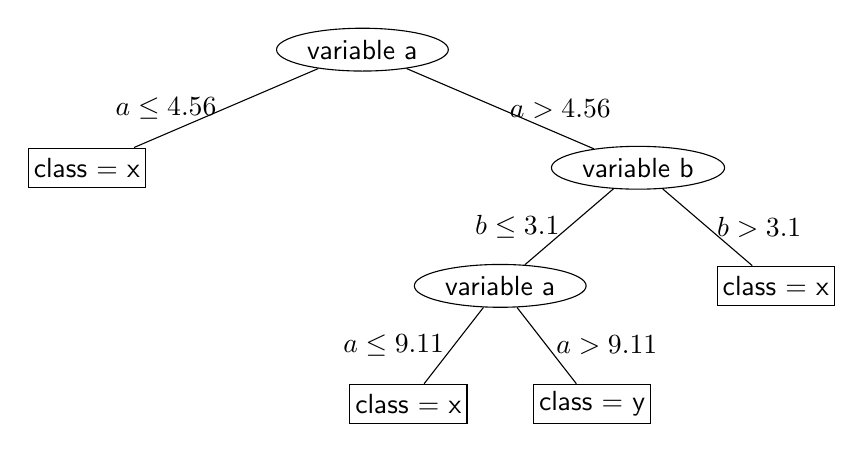
\begin{tikzpicture}[level/.style={sibling distance = 7cm/#1}]
\usetikzlibrary{shapes}
\usetikzlibrary{arrows}
\node [arn_d] {variable a}
    child{ node [arn_c] {class = x} edge from parent node[left] {\(a \le 4.56\)} }
    child{ node [arn_d] {variable b}
        child{ node [arn_d] {variable a}
            child{ node [arn_c] {class = x} edge from parent node[left] {\(a \le 9.11\)} }
            child{ node [arn_c] {class = y} edge from parent node[right] {\(a > 9.11\)} }
            edge from parent node[left] {\(b \le 3.1\)}
        }
        child{ node [arn_c] {class = x} edge from parent node[right] {\(b > 3.1\)} }
        edge from parent node[right] {\(a > 4.56\)}
    }

;
\end{tikzpicture}
\end{center}
\end{figure}

The decision trees used by random forests are constructed by randomly
selecting a certain number of input variables as configured by the parameter
\texttt{mtry} for each node.
The algorithm then selects the best split on one of these input
variables as the node's criterion, using what is called an optimality criterion.
This process is repeated for every child node until a node is reached
which only matches records in the dataset satisfying a stop criterion.
This node becomes a leaf node.
This is described as growing a tree maximally.
It ensures that each decision tree has a high strength,
meaning no decision tree outputs wrong predictions for the subsets of data
it matches. \cite{breiman2001random}

As a component classifier to an ensemble learning algorithm,
every decision tree should be different from the other decision trees in
the ensemble, i.e. the decision trees should be diverse,
to cover a wide range of possible interactions between the input data,
i.e. hypotheses.
This is commonly described as the trees being uncorrelated.
Tree strength and inter-tree correlation are what the prediction accuracy
of random forests depends on. \cite{breiman2001random}

The procedure by which decision trees are grown is modified in some
variants of random forests.
The PERT (perfect random tree) algorithm \cite{cutler2001pert} for example doesn't perform a
search for the best split on a random selection of input variables,
but selects variable and threshold at random.
The RFW (random feature weights) algorithm \cite{maudes2012random} searches all variables but attaches random
weights to them, and the DRF (dynamic random forests) algorithm \cite{bernard2012dynamic} influences the
decision tree creation by a procedure inspired by boosting.
Other variants, e.g. \citeA{van2012accelerating}, change this procedure to
grow smaller or more balanced trees, to meet performance or
hardware requirements.

\subsection{Random Forests}
As has been described in the sections on ensemble learning and decision trees,
random forests build ensembles of decision trees.
This process depends on two parameters: the ensemble size, commonly called
\texttt{ntree}, and the randomisation parameter \texttt{mtry}.
Actually, random forests depend on another parameter,
the state of a random number generator, but being random,
it doesn't and usually shouldn't be specified.

The following is an exemplary implementation of the random forest algorithm
roughly following the original version by \citeA{breiman2001random}.
I wrote this implementation to illustrate the simplicity of random forests,
as well as its components.
The implementation uses entropy instead of the Gini index as
optimality criterion, a naive stop criterion only capable of handling
perfectly partition-able data, and lacks variable importance measures.
In reference to the higher level programming languages mentioned
in the introduction, the following source code is written in a Lisp
dialect called Clojure \cite{wpCLOJURE}, and uses a functional data structure
called \emph{zipper} \cite{huet1997zipper} for efficient tree construction.

For every tree in a random forest ensemble, the algorithm first draws a
bootstrap sample from the dataset.
The following \texttt{bootstrap} function takes a vector of rows as input
and returns an equally large bootstrap sample and the corresponding out-of-bag data.

\begin{figure}[H]
\caption{The \texttt{bootstrap} function.}
\begin{minted}[baselinestretch=1]{clojure}
(defn bootstrap [dataset]
  (let [n (count dataset)
        s (repeatedly n #(rand-int n))
        d (set (map #(nth dataset %) s))
        o (set (filter (comp not d) dataset))]
    {:dataset d :oob o}))
\end{minted}
\end{figure}

For each node in a tree the algorithm first has to select the rows in the dataset
that match all criteria up to the given node.
The following \texttt{select} function takes a vector of rows, and a tuple of a variable name
and a split value as input, and returns lists of the matching and the not matching rows.

\begin{figure}[H]
\caption{The \texttt{select} function.}
\begin{minted}[baselinestretch=1]{clojure}
(defn select [[v s] dataset]
  (let [l (reduce (fn [acc t]
                    (if (<= (get t v) s) (conj acc t) acc))
            #{} dataset)
        r (set (filter (comp not l) dataset))]
    [l r]))
\end{minted}
\end{figure}

For each node the algorithm then progresses to check whether the node should be split,
and if so, selects the best split out of a random selection of split variables.
The \texttt{splits} function takes a dataset and \texttt{mtry} as parameters and
returns all splits as tuples of variable name and split value.
The \texttt{best-split} function calculates the entropy for every split and applies
the best split to two datasets simultaneously (sample data and out-of-bag data).
This is done because both sample and out-of-bag data are stored in each node to
simplify the decision tree construction and the error estimate calculation.
Since Clojure features immutable data structures this increases memory usage only negligibly.

\begin{figure}[H]
\caption{The functions \texttt{splits} and \texttt{best-split}.}
\begin{minted}[baselinestretch=1]{clojure}
(defn splits [dataset mtry]
  (let [vs (filter (partial not= :class) (keys (first dataset)))
        n (count vs)
        vs (if (<= mtry n) (take mtry (shuffle vs)) vs)]
    (reduce (fn [acc v]
              (reduce (fn [acc t]
                        (conj acc [v (get t v)])) acc dataset))
            #{} vs)))

(defn best-split [dataset oob mtry]
  (let [[_ s l r]
    (first (sort (map (fn [s] (let [[l r] (select s dataset)]
                                [(entropy l) s l r]))
                      (splits dataset mtry))))]
    (let [[oobl oobr] (select s oob)]
      [s (set l) (set r) (set oobl) (set oobr)])))
\end{minted}
\end{figure}

The \texttt{extend-node} function uses \texttt{leaf?} to check whether the node
should be split, does so if necessary using the \texttt{best-split} function, and
hands down the appropriate datasets to the child nodes.

\begin{figure}[H]
\caption{The stop criterion \texttt{leaf?} and the node splitting function \texttt{extend-node}.}
\begin{minted}[baselinestretch=1]{clojure}
(defn leaf? [dataset] (= (entropy dataset) 0.0))

(defn extend-node [{:keys [dataset oob] :as node} mtry]
  (if (leaf? dataset)
    (merge node
           {:class (or (first (first (sort-by val >
                         (frequencies (map :class dataset)))))
                       :unknown)})
    (let [[s l r oobl oobr] (best-split dataset oob mtry)]
      (merge node
             {:criterion s :left  {:dataset l :oob oobl}
                           :right {:dataset r :oob oobr}}))))
\end{minted}
\end{figure}

The following \texttt{rf-train} function is the top-level function responsible for
building the ensemble of decision trees.
It creates \texttt{ntree} decision tree root nodes, each with its own sample
and out-of-bag datasets, walks through each tree using a zipper,
and invokes the \texttt{extend-node} for each node in every tree.
The different trees in the ensemble are constructed in parallel using \texttt{pmap},
distributing the work among all available processor cores.

\begin{figure}[H]
\caption{The \texttt{rf-train} function.}
\begin{minted}[baselinestretch=1]{clojure}
(defn rf-train [dataset ntree mtry]
  (set (pmap (fn [sample]
         (loop [loc (zip/zipper
                      (fn [node] true)
                      #(if (:left %)
                        (seq [(:left %) (:right %)]))
                      (fn [node children]
                        (with-meta
                          (merge node
                                 {:left  (first children)
                                  :right (second children)})
                          (meta node)))
                      sample)]
           (if (zip/end? loc) (zip/root loc)
             (recur
               (zip/next (zip/edit loc extend-node mtry)))))
         (repeatedly ntree #(bootstrap dataset)))))
\end{minted}
\end{figure}

The \texttt{rf-predict} is another top-level function.
It takes a random forest and a row of input values, and returns the outcome as
predicted by the random forest.

\begin{figure}[H]
\caption{The \texttt{rf-predict} function.}
\begin{minted}[baselinestretch=1]{clojure}
(defn rf-predict [forest features]
  (let [eval-tree
          (fn eval-tree [tree]
            (if (:class tree) (:class tree)
              (if (let [[v s] (:criterion tree)]
                    (<= (get features v) s))
                  (eval-tree (:left tree))
                  (eval-tree (:right tree)))))]
    (first (first
      (sort-by
        val > (frequencies
                (filter (partial not= :unknown)
                        (pmap eval-tree forest))))))))
\end{minted}
\end{figure}

The following top-level function \texttt{rf-error} calculates the random forest's
error estimate by invoking \texttt{tree-error} for each tree in the ensemble.
The \texttt{tree-error} function uses the out-of-bag data stored in each leaf node
and compares it to the predicted outcome of that leaf.
Since this implementation only handles noiseless datasets, the error estimate
returned by \texttt{rf-error} will only ever be zero.

\begin{figure}[H]
\caption{The \texttt{rf-error} and \texttt{tree-error} functions calculate the error estimate.}
\begin{minted}[baselinestretch=1]{clojure}
(defn tree-error [tree]
  (let [cls (:class tree)]
    (cond (nil? cls) (+ (tree-error (:left tree))
                        (tree-error (:right tree)))
          (= cls :unknown) 0
          :else (count
                  (filter (partial = cls) (:oob tree))))))

(defn rf-error [forest]
  (/ (reduce + 0
       (pmap #(/ (tree-error %) (count (:oob %))) forest))
     (count forest)))
\end{minted}
\end{figure}

For information on how to use this implementation of random forests,
see example and instructions in the appendix.

\subsubsection{Parameters}
The two parameters random forests depend on, the size of the forest
\texttt{ntree} and the number of randomly selected variables at each node
\texttt{mtry}, are problematic,
in that users set them according to one recommendation or another,
or just use the default settings, which again can differ from implementation
to implementation.
Furthermore, not every dataset is best learned by random forests using the
same settings.
This lack of a standard way to determine the parameter values makes it hard
to compare the accuracy of different methods.
The comparative study by \citeA{banfield2007comparison} gives an
illustrative overview over the datasets used in previous publications,
among which are \citeA{breiman2001random} and \citeA{dietterich2000ensemble},
that each used ensemble sizes of 50-200, and applied the algorithms being
compared to 18-27 datasets.
In each case the authors concluded that their method was superior to the
other methods in the study.
However, the more recent study by \citeA{banfield2007comparison} found
“no stat. sig. improvement over bagging in 38 of 57 data sets”
when ensemble sizes of up to 1000 trees where used.
The study also concludes that bagging with an ensemble size of 1000 and
random forests with the randomisation parameter set to the
binary logarithm of the number of input variables were the best methods.
The study by \citeA{banfield2007comparison} also suggests a mechanism
to determine the best size of the ensemble automatically.
Methodologically, this would be a welcome improvement, because it eliminates
one way researchers can fiddle with the outcome of their calculations,
and because it would ensure better results due to the usually larger
ensemble sizes.
In defense of older studies, like those by \citeA{breiman2001random} and
\citeA{dietterich2000ensemble}, one has to mention that
computers back then weren't as powerful.
\citeA{breiman2001random} mentions run times for random forests of 4 minutes
and 3 hours for Adaboost when building ensembles of size 100,
while I can execute all examples in the paper by \citeA{strobl2009introduction}
in well under 10 seconds on one core running at 3.40 GHz, consuming about 180 Mb
of memory.

The second parameter of random forests is the randomisation parameter
\texttt{mtry} which controls how many variables are being selected randomly
at each decision tree node to search for an optimal split.
If \texttt{mtry} is set to the number of variables, random forest becomes
bagging as proposed by \citeA{breiman1996bagging}.
Common choices for \texttt{mtry} are 1, 2, and other small values in
older studies, e.g. \citeA{breiman2001random}, and the square root of n,
or the binary logarithm of n, with n being the number of input variables,
becoming increasingly popular in newer literature, e.g.
\citeA{strobl2009introduction}.
As mentioned above, using the binary logarithm of the number of
input variables is indeed the best choice for most datasets
\cite{banfield2007comparison}.
However, depending on the dataset and the ensemble size, \texttt{mtry}
needs to be chosen differently.
For example in studies of genetics, where the dataset often includes many
irrelevant input variables in addition to the dataset being a
“small n large p case”, it is necessary to use a larger value
for \texttt{mtry}, else some variables might never be used in the ensemble
at all \cite{strobl2009introduction}.
It might be interesting to consider choosing \texttt{mtry} automatically.
One way to do this, is to systematically try different values for \texttt{mtry}
and choose the best one using cross-validation \cite{psymeth}.
According to \citeA{bernard2008forest} a greedy search or choosing one of
the values discussed above is the usual approach in the literature.
The same paper shows, that this doesn't have to be the case, by demonstrating
a "push-button" method that automatically derives a suitable value for
\texttt{mtry} and "is at least as statistically significant as the original"
\cite{bernard2008forest}.

\subsubsection{Out-of-bag Data}
Because random forests are based on bagging and use bootstrapped samples,
each tree has a set of approximately one third of the original dataset
that has not been used to grow the tree.
This set can be used to test the prediction accuracy of each tree,
and the prediction accuracy of all trees can then be averaged to give an
error estimation of the entire random forest.
This out-of-bag error estimation is more precise than the naive error
estimate, which is using all of the dataset \cite{strobl2009introduction}.
This said, one should not forget that out-of-bag data isn't the
same thing as a genuine test dataset.
Depending on the size of the dataset, and the size of the ensemble,
the downsides
of bootstrapping might shine through, and lead to an underestimation of
the prediction accuracy.

\subsubsection{Variable Importance}
As has been mentioned above, random forests have a built in variable
importance measure, which is calculated by permutating one input variable
in the out-of-bag data of every tree, and calculating a new error estimate.
The difference between the out-of-bag error estimates with and without
randomly permutated input variable is the variable importance.
The more important a variable is, the more drastically the prediction error
increases when the variable is being randomised.
The variable importance measure is sometimes scaled, i.e. z-standardised,
but because it strongly depends on the parameter of random forests,
it's not possible to compare these variable importances across studies,
hence there is little use in doing so, and the practice only encourages
problematic comparisons across studies \cite{strobl2009introduction}.

The idea behind this way of calculating variable importances is,
that one would like to compare a prediction model with and without a
particular input variable to measure the variable's impact.
Obviously, one can't ignore all trees that incorporate a variable,
because each tree incorporates multiple input variables, and their impact
on the prediction would be modified too.
By randomly permutating the values of an input variable,
the variable's characteristics don't change, but the connection to the
output variable is broken.
However, according to \citeA{strobl2007bias} the variable importance might
still depend on which variable is being measured, because the
variable importance measure is biased towards variables with many categories
and variables with many missing values.
Numeric variables usually have as many different values as there are records
in the dataset, meaning that their importance measure is greatly biased due
to the large number of “categories”.
Fortunately, this can be fixed, but “Only when subsamples drawn without
replacement, instead of bootstrap samples, in combination with unbiased
split selection criteria, are used in constructing the forest, can the
resulting permutation importance be interpreted reliably”
\cite{strobl2007bias}, and correlated input variables still are
problematic.
The R package \texttt{party} includes two functions, \texttt{ctree} and
\texttt{cforest}, that use a different method for split selection and aren't
affected by this bias.
Therefore, \texttt{cforest} actually uses another variable importance termed
“conditional variable importance” \cite{strobl2008conditional}.
Correlated variables can be problematic, because trees that include a
pair of correlated input variables are less affected by the random
permutation of one of them.
Conditional variable importance considers these correlations.
However, \citeA{gromping2009variable} argues, that this problem can't be avoided
as long as \texttt{mtry} is smaller than the number of input variables,
and that considering all input variables, i.e. bagging,
“might already go a long way” towards remedying the problem,
although due to the “large p small n case”, “unbiased estimation of all
coefficients is impossible” in any case.

Another problem that the variable importance measure can be affected by,
is that some variables might not be well represented in a random forest.
This can be due to a small setting for \texttt{mtry} and or \texttt{ntree}
in the presence of many irrelevant input variables, as often is the case
in genetics datasets, or if variables show perfect higher order effects,
i.e. interaction effects, but no main effects.
The latter is called the XOR problem.
It is important to note, that random forests with a different split selection
algorithm don't have to be affected by this, e.g. PERT \cite{cutler2001pert}.

Last but no least, both \citeA{strobl2009introduction} and
\citeA{gromping2009variable} see one of the advantages of random forests in
their variable importance measure.
\cite{gromping2009variable} compares linear variable importance measures
with the one built into random forests, and finds that the latter are
heavily dependent on the mtry parameter.
The larger \texttt{mtry} is, the better the importance estimates become.
Variable importance measures are used to select input variables for a simpler
model, e.g. a generalised liner model, which is more interpretable than a
forest of decision trees \cite{strobl2009introduction}.
Variable importance measures also are the probably only simple way to
“shed some light into the black box of random forests”
\cite{gromping2009variable}.
An alternative, but rather naive way to estimate variable importance is to count
the occurrence of a variable over all trees \cite{strobl2009introduction}.
Other imaginable ways to estimate variable importance would be to use
algorithms that analyse the structure of each decision tree.
Another interesting point to make is, that random perturbation of an input
variable could in theory be used as part of many other models, including but
not limited to generalised linear models, because although
this isn't very useful in the case of generalised linear models,
many other complex models are similarly difficult to tease apart, e.g.
neural networks.

The way variable selection based on variable importance measures is
being done, is by finding variables whose randomisation led to an improvement
in prediction accuracy.
These improvements are just random effects, and function as an indicator
for which variable importances are within the band of random fluctuations,
and which are true indicators for important variables.

\subsubsection{Regression}
Random forest can not only be used for classification, but also for regression.
To produce the numeric output values necessary for regression,
the vote on the most popular output class in the forest is replaced by the
calculation of an average over all tree outputs.
One problem with regression using random forests is that more decision trees
end up covering the middle range of values of output variable.
This means that the prediction accuracy is good in the middle of the range
of values, but that the predictions for extremer values become more and more
inaccurate \cite{zhang2012bias}.
The same paper also suggests five ways to estimate and reduce this problem.

\subsubsection{Overfitting}
Overfitting \cite{wpOF} is the situation where an algorithm learns the
example dataset well enough to not only reproduce the underlying rules,
but to also reproduce the random errors in the dataset.
This is also called \emph{generalisation error}, since the algorithm
generalises errors in the data by deriving rules for them.
Random forests grow optimal decision trees, meaning they try to represent
each bootstrapped sample perfectly.
Except for the case where different records in the sample have the same
values in their input variables, but different values in their output variable,
this leads to decision trees which represent the sample perfectly,
including all errors.
The advantage of ensemble learning is that by combining decision trees grown
for different samples, and constructed using different random split selections,
these errors are cancelled out.
However, this also means that there is an upper bound on how accurate
random forests can become depending on the noise present in the dataset.
Of course, this only applies if the trees in an ensemble are reasonably
diverse, i.e. uncorrelated \cite{breiman2001random}.
An analysis by \citeA{liu2005maximising} showed that the generalisation error
is at its lowest when the tree ensemble is maximally diverse,
and that bootstrapping tends to limit tree diversity.

Different variants of random forests try to grow random forests on data
that is less prone to noise.
FRF stands for \emph{Fuzzy random forests}, and is a method described by
\citeA{bonissone2008fuzzy}.
FRF use what are called \emph{fuzzy sets} to represent the data in the dataset,
and to build their decision trees on top.
The advantages of this approach are that the resulting FRF are more immune
to noise, and \citeA{cadenas2012extending} extend this framework to
handle missing data too.
Another attempt at constructing random forests from smoother data are
rotation forests by \cite{rodriguez2006rotation}, which use
principal component analysis, or PCA, to find derived input variables that
represent the input dimensions better.
Although linear combinations of input dimensions aren't the same thing
as noise, since datasets are of a limited size, and decision trees
might well fail to tease out the interactions between all pairs of input
variables, they will look like noisy input data if the decision trees
don't catch on.
Because better input dimensions lead to better splits, and to more
uncorrelated random variable selections, rotation forests are often more
accurate than random forests \cite{rodriguez2006rotation}.

\subsubsection{Optimality Criterion}
Random forests construct the underlying decision trees by selecting the
best split at each node from a number of randomly selected variables.
To compare the different possible splits, an optimality criterion gets
calculated for each split.
The most commonly used criterion is the Gini index.
The Gini index is “a measure of statistical dispersion developed by the
Italian statistician and sociologist Corrado Gini” \cite{wpGINI},
but it can also be used as a measure of entropy.
The latter is how it is used in random forests.
As has been mentioned in the section on variable importance, the fact that
the Gini index is biased towards variables with many different values
is problematic.
Another common optimality criterion is entropy, although it suffers from
the same bias towards variables with many different values.
The point of using an optimality criterion in the first place is,
to grow trees using an impurity reduction algorithm, i.e. to select the split
which returns the least dispersed subsets is selected recursively at each node.

A huge disadvantage of using an optimality criterion is the computational cost
one has to pay.
Trees which use random splits are much faster to grow, e.g. PERT ensembles
are claimed to be two orders of magnitude faster than the classical
random forests \cite{cutler2001pert}.
\citeA{cutler2001pert} indicate that despite its simplicity,
"[...] PERT falls within the range of the other three methods.", meaning
Adaboost and two random forest variants (different \texttt{mtry}),
in terms of its prediction accuracy.


\subsection{In Search of the Super-Forest}
The following section will look at some of the random forest variants that
have already been mentioned above. It concludes by calling for a more
user-friendly random forest variant, which combines many of the features of
the proposed variants, and is tailored to the less technically adept users
in the social sciences.

\subsubsection{Alternative: PERT}
PERT, a variant in the random forests framework was developed
by \citeA{cutler2001pert}.
The nice feature of PERT is that its strong reliance on randomness gives
it a simple structure that is easier to describe and implement than the
classical random forests by \citeA{breiman2001random}.
In fact, PERT is simple enough that its algorithm is completely described
in the following quote from \citeA{cutler2001pert}:

\begin{quotation}
The perfect random tree ensemble, PERT, is so named because the PERT base
learner is a random tree classifier that fits the training data perfectly.
The PERT base learner is constructed by first placing all data points in
the root node.
At each step of the tree construction, each non-terminal node is split by
randomly choosing two data points from the node until these two belong to
different classes.
Let \( x = (x_{1} , . . . , x_{p} ) \) and \( z = (z_{1} , . . . , z_{p} ) \).
If this is not possible, all the data points in the node must be from the
same class and the node is terminal.
Now, randomly choose a feature on which to split, say feature j, and split
at \( \alpha x_{j} + (1 - \alpha) z_{j} \), where \( \alpha \) is generated
from a uniform(0,1) distribution.

Ties are taken care of by repeating the procedure until a definitive
split is obtained.
If no such split is found after 10 tries, the node is declared to be
terminal (so in this case, the tree would not perfectly fit the data).
To form an ensemble, PERT base learners can be combined by simply fitting
many PERT base learners to the entire training set and voting these
classifiers.
Alternatively, PERT base learners can be combined by bagging
\cite{breiman1996bagging}.
In this case, the PERT base learner is fit to many bootstrap samples
from the training data and these classifiers are combined by voting.
\end{quotation}

On the one hand, bagging is not required, because PERT doesn't depend on
randomness introduced through bootstrapping.
On the other hand, bagging can be used if one requires out-of-bag
error estimates or variable importance measures, and as a way to deal
with ties in the dataset.
As \citeA{liu2005maximising} have indicated, bootstrapping might lead
to less diverse trees, thus it should not be used unless one requires
these features.

The advantage of PERT over random forests is speed.
\citeA{cutler2001pert} compare the different runtimes of classical random
forests construction, as described in \citeA{breiman2001random}, and PERT
to find the latter to be faster by two orders of magnitude,
while providing similar accuracy in prediction.
Of course, there are other advantages too:
The absence of a variable selection criterion means that PERT doesn't suffer
from the bias introduced by it, thus, variable importance estimates are less
affected.
An instance where the use of a selection criterion is especially problematic
is the XOR problem mentioned above in the section on variable importance.
Since PERT forests don't depend on an optimality criterion to select their
splits, PERT has the advantage of being able to deal with perfect
interaction effects.
A disadvantage is that PERT forests are even more difficult to interpret than
the classical random forests, but since this is rarely tried anyway,
it probably doesn't matter much in practice.
It is important to mention however, that PERT can only be used for
classification,
since its base learner fits the training data perfectly, applying PERT to
regression would “drastically overfit the data” \cite{cutler2001pert}.

PERT isn't the only random forest variant that emphasises randomness in its
algorithm for growing trees.
\citeA{geurts2006extremely} suggested what they call \emph{extremely randomised trees}.
Despite their name, extremely randomised trees are actually closer to the
trees of random forests by \citeA{breiman2001random} than PERT, 
in that they do select the best split from a random subset variables of size \texttt{mtry},
although the actual split value for each variable is generated randomly.
Furthermore, they don't fit the data perfectly, but allow the user to
choose a "minimum sample size for splitting a node" \cite{geurts2006extremely}.
This parameter, called \emph{smoothing strength} by \citeA{geurts2006extremely},
prevents overfitting in noisy datasets, and allows the user to configure the
behaviour of the algorithm in order to adapt
the random forest algorithm to dataset at hand.

\subsubsection{Alternative: Fuzzy random forests}
Fuzzy random forests by \citeA{bonissone2008fuzzy} use input variables
encoded as fuzzy sets.
Fuzzy sets \cite{wpFS} model membership to a category by a value between
one and zero, while fuzzy logic \cite{wpFL} allows to reason using fuzzy data:
For example, a day with a temperature of 45 degrees Celsius is to 100\% a
hot day, and to 0\% a cold day, while a day with 15 degrees Celsius might
belong to the label cold day by 40\% and to hot day by 60\%.
The advantage of using fuzzy sets is the added flexibility of representing
uncertainty.
\citeA{cadenas2012extending} extended fuzzy random forests to handle
missing data, thus making fuzzy random forests even better at representing
real world data.

\subsubsection{Alternative: Rotation forests}
Rotation forests use principle component analysis to transform
the dataset before creating the ensemble of decision trees.
"Principal component analysis (PCA) is a mathematical procedure that uses
an orthogonal transformation to convert a set of observations of possibly
correlated variables into a set of values of linearly uncorrelated variables
called principal components." \cite{wpPCA}
Rotation forests have been suggested by \citeA{rodriguez2006rotation}.
Rotation forests are created by calculating a PCA (principal component analysis)
on the bootstrap sample of each tree prior to building the tree.
To apply PCA, the input variables are split into subsets and rows matching
randomly selected values of the output variable are removed.
The PCA coefficients for each subset are then arranged into the rotation matrix
used to transform the sample before building the tree.
This means that another parameter, the size of input variable subsets, is required.
Rotation forests significantly outperform random forests, bagging, and
boosting on many datasets, but due to the transformation of the dataset,
rotation forests do not provide variable importance measures \cite{rodriguez2006rotation}.

The transformation of the input data leads to less correlation between trees,
and to improved prediction accuracy, which \citeA{rodriguez2006rotation}
demonstrate with the help of diversity-error diagrams.

\subsubsection{Future Random Forests}
The different algorithms in the random forest framework have been developed
iteratively, with each improvement or variation picking up one problem to
improve on.
The criterion for success has been beating the base algorithm.
Similar to how the scientific method has become a competition between
researcher and randomness, the field of research on random forests seems
to be plagued by comparisons between the old and the new forests.
It might be worth the effort to step back from the specifics for a moment
and look at the principle behind random forests.

Every variant in the random forests framework is an ensemble of trees.
Beyond that there seems to be nothing that may not be changed.
Two questions that naturally follow from this are:

\begin{APAenumerate}
\item Can a random forest incorporate all of the developed features?
\item How does one prioritise the different features and problems?
\end{APAenumerate}

Most of the suggested improvements and variants have taken the original
random forest algorithm and changed some part of it. Since the changes of
the different variants discussed in this report don't overlap, combining
them should certainly be possible.
The more interesting question is the second.
This report has mentioned many problems of random forests, for example the
problem of parameter selection.
To increase the reach of random forests in general, and particularly in
the social sciences, the parameter situation needs to be resolved, because
not every researcher can include a simulation study just to show that his
methods are not flawed.
An accepted solution to this problem is to tune the parameters using cross-validation.
While this is a good solution for most applications, it does lead to an
underestimation of the error estimate, which can be problematic in some cases.
Obviously this can be fixed by setting aside a dedicated test dataset, but
compiling an even larger dataset is often unpractical, since real world datasets
aren't cheap to compile.
By including the suggestions of \citeA{banfield2007comparison} regarding
\texttt{ntree} and \citeA{bernard2008forest} regarding \texttt{mtry}
a new random forest variant could be completely parameterless.
Alternatively, a new random variant could use PERT to get rid of the
parameter \texttt{mtry} and some of the bias in the variable importance
measure.
Both approaches do not require additional data.

Obviously, there is no single best solution, but this doesn't make unifying
random forest variants a futile task.
The simpler and safer a method is to use, the wider it will spread, and by
spreading a good default method, all of scientific research will benefit.

\newpage
\section{Method}
\subsection{Selection of Papers}
I started my research on random forests by reading the
introductory paper suggested by my supervisor titled
\emph{An introduction to recursive partitioning: Rationale, application
and characteristics of classification and regression trees, bagging and
random forests} \cite{strobl2009introduction}.
I then searched the research databases \emph{PsychARTICLES} and
\emph{PsychINFO} querying for random forest and limiting my results
to the last two years.
I only considered papers that focus on random forests and
dismissed almost all papers where random forests are merely used as a
method of analysis.
I also used \emph{Google Scholar} to look for the more technical
publications outside the field of psychology.
I searched for combinations of \emph{random forest}, \emph{comparison},
\emph{analysis}, and \emph{ensemble}.
I also included keywords seen in interesting titles, like \emph{fuzzy},
\emph{perfect}, \emph{full}, \emph{balanced}, \emph{extremely}, and
\emph{rotation}.
I then looked for some of the referenced publications I read about in the
papers found as mentioned above, and included \citeA{strobl2008conditional},
\citeA{ho1998random}, \citeA{breiman1996bagging}, \citeA{freund1995decision},
and \citeA{long2010random}.

The final criteria for inclusion were the online availability of a freely
downloadable PDF-file, which thanks to \emph{Google Scholar} often turned
out to be no problem at all, and my decision on the topic of
this report.
It turned out, that while Google Scholar is convenient to find freely
downloadable PDF-files, its citations aren't up to par.

A lot of the information in the fields of computer science, artificial
intelligence, machine learning, databases, and especially programming
I acquired through different means in the last ten years.
As I can't remember the original sources, I include the pages
on Wikipedia and a few books, e.g. \citeA{borzlinreg, barberMLC, haykin, qai},
which I used to refresh my memories.

\subsection{Aim and Structure of the Paper}
Possible options for this topic were the presentation of
exemplary uses of random
forests, the discussion of strengths and weaknesses, and any of the more
specialised variants.
During my research I had the impression, that there were serious
differences in the understanding of random forests among researchers,
and even among designers of improved variants.
A study comparing different decision tree ensemble techniques also confirmed
this expression by saying that many of the commonly used methods of comparison
weren't robust enough for use with random forests \cite{banfield2007comparison}.

Because of this fuzziness, I decided on a different focus, to write
a very broad - big picture - introduction to random forests.

\newpage
\section{Discussion}
\subsection{Random forests}
Random forests are diverse.
There is no “the random forest” method, but rather a wide spectrum of
methods that all use similar principles.
Random forests are accurate and very powerful, because they can be used
on almost any dataset.
The way a random forest is grown lends itself to be run on multiple processor 
cores at once, as the
small exemplary implementation demonstrates, which is an important criterion
for anyone who wants to analyse large datasets.
On top of that, they are easy to implement and don't require a sophisticated
mathematical understanding.
In fact, a lot of the random forest variants have been developed by combining
known concepts and later proving the viability using  a comparison of methods
study on real-world and simulated datasets.

However, it has to be said that random forests can be problematic,
because they appear to be easy to use, but expose a lot of their
inner workings to the user.
The user shouldn't have to worry about parameters, and how they interact
with a dataset to introduce bias in error estimates and
variable importance measures.
In studies where only small ensembles are used, one has to wonder if the
researcher didn't just get lucky with his random number generator's seed value.
In some ways \citeA{banfield2007comparison} can be seen to ask the same question,
since the claimed significant improvement in prediction accuracy of many methods
disappear when the comparisons are conducted more rigorously.

The very ease with which random forests can be implemented and changed,
should lead to a more thorough study of their qualities,
and the qualities of random forest variants, but this seems not to be the case.
Most comparisons pitch a specific variant against the random forests
of \citeA{breiman2001random}, bagging \cite{breiman1996bagging}
and Adaboost \cite{freund1995decision}.
One of the factors for this I believe to be the lack of a standardised
and automatic testing infrastructure, which would simplify the development
and testing of new algorithms.

\subsection{Methods research}
If the datasets and protocols for measuring and comparing algorithms were
developed first and standardised, new algorithms could be measured by the
push of a button.
Authors wouldn't have to use half of their publication
to describe the datasets used in a comparison.
Furthermore, by combining the knowledge of the particularities of a dataset,
especially real-world datasets, authors would have access to immediate
indications on why their method might be particularly good or bad when applied
to a certain type of data.
Such a standardised test repository would also lighten the load of all the
researchers just using random forests as a tool.
They wouldn't have to explain why they choose a particular variant based on
their incomplete knowledge of machine learning, but could just refer to
a standard.
This would certainly be beneficial for research in general, but one doesn't have
to stop there.
By standardising research methods, their development and comparison
in general, it also becomes easier to replicate a study's results using
different methods on the same dataset, and the datasets of a study can
be included in the corpus of test-sets for future testing of methods.
One of the more well-known repositories of datasets is the \emph{UCI Machine Learning Repository}
\cite{UCIrepo}, but unfortunately many researchers hesitate to donate their
datasets to such a repository.

The “Methods” section of a study and the research methods mentioned in it,
shouldn't be separate, because relying on a particular version of a particular
tool to decide over the significance of findings is not very scientific.
Unfortunately, this happens:
Researchers are very careful when selecting theories from their own field,
but sometimes flagrantly refer to "default settings" with no further detail,
when they use an implementation of a method,
just because software or random forests are not their field.
Default values in implementations do change, and these changes sometimes
happen for a reason.
It should be possible to check if a study is affected by this change,
and reevaluate it if necessary.
In keeping with the artificial intelligence origins of machine learning,
one can envision a display of a huge dependencies graph with
red and green lights representing the state of research fields.
Computers would do the automated rechecking of past studies as soon as
new datasets or new methods become available, and notify researchers
when the premises of their work or field of study were refuted.
Computers could also publish requests for dataset and new methods,
when they detect methodical weaknesses and other “anomalies”.

Obviously, this is quite a different topic than random forests, but the
field of research on random forests nicely illustrates how some of the
problems play out.
Just because \citeA{breiman2001random} uses certain parameters for the
comparison, this doesn't mean that the parameters are a good choice when
demonstrating the powers of a new random forest variant.
Since random forests all roughly take the same format of input data and
parameters, it should be trivial to cross-validate all findings with all
datasets and all variants, but as it stands this is still difficult to do in practice.
One doesn't know if another study like \citeA{banfield2007comparison}
overturns random forests in the near future by finding another method to be
superior.
For most researchers in other fields it's thus a safer bet to stick to
traditional methods.
Unfortunately, this often means to ignore problems with many input variables,
or not daring to invent models with complex interactions,
which are difficult to represent using traditional methods.

\newpage
\section{Appendix}
The following Clojure source code is the complete version of the
exemplary implementation of random forests discussed earlier in this paper.
To run the examples, install the \texttt{Leiningen} build system
\cite{leiningen}, save the following source code to the indicated files,
and start up the interactive \emph{REPL} (read eval print loop).

\begin{figure}[H]
\caption{Shell commands to start the Clojure REPL.}
\begin{minted}[baselinestretch=1]{bash}
$ cd rf/
$ lein deps
$ lein repl
\end{minted}
\end{figure}

Once this is done, provided no unexpected errors have occurred,
the random forest implementation can be used as follows.
Please refer to the source code below for information on the
format of the dataset.

\begin{figure}[H]
\caption{An example interaction in the REPL illustrating how to use the random forest implementation.}
\begin{minted}[baselinestretch=1]{clojure}
user=> (require '[rf.core :as r])
nil
user=> (def forest (r/rf-train r/sample 150 3))
#'user/forest
user=> (every? #(= (r/rf-predict forest (dissoc % :class)) (:class %))
  #_=>         r/sample)
true
user=> (r/rf-error rf)
0
user=> (exit)
Bye for now!
\end{minted}
\end{figure}

\newpage
\begin{minted}[baselinestretch=1]{clojure}
; file: rf/project.clj

(defproject rf "1.0.0-SNAPSHOT"
  :description "An examplary random forest implementation."
  :dependencies [[org.clojure/clojure "1.5.1"]])
\end{minted}

\newpage
\begin{minted}[baselinestretch=1]{clojure}
; file: rf/src/rf/core.clj

(ns rf.core
  (:require [clojure.zip :as zip]))

(def sample [
  {:a 0 :b 0 :c 0 :d 0 :class :0} {:a 1 :b 0 :c 0 :d 0 :class :8}
  {:a 0 :b 0 :c 0 :d 1 :class :1} {:a 1 :b 0 :c 0 :d 1 :class :9}
  {:a 0 :b 0 :c 1 :d 0 :class :2} {:a 1 :b 0 :c 1 :d 0 :class :a}
  {:a 0 :b 0 :c 1 :d 1 :class :3} {:a 1 :b 0 :c 1 :d 1 :class :b}
  {:a 0 :b 1 :c 0 :d 0 :class :4} {:a 1 :b 1 :c 0 :d 0 :class :c}
  {:a 0 :b 1 :c 0 :d 1 :class :5} {:a 1 :b 1 :c 0 :d 1 :class :d}
  {:a 0 :b 1 :c 1 :d 0 :class :6} {:a 1 :b 1 :c 1 :d 0 :class :e}
  {:a 0 :b 1 :c 1 :d 1 :class :7} {:a 1 :b 1 :c 1 :d 1 :class :f}])

(defn bootstrap [dataset]
  (let [n (count dataset)
        s (repeatedly n #(rand-int n))
        d (set (map #(nth dataset %) s))
        o (set (filter (comp not d) dataset))]
    {:dataset d :oob o}))

(defn select [[v s] dataset]
  (let [l (reduce (fn [acc t]
                    (if (<= (get t v) s) (conj acc t) acc))
            #{} dataset)
        r (set (filter (comp not l) dataset))]
    [l r]))

(defn entropy [dataset]
  (let [n (count dataset)
        p (map #(/ % n) (vals (frequencies (map :class dataset))))
        l #(/ (Math/log %) (Math/log 2))]
    (* -1 (reduce #(+ %1 (* %2 (l %2))) 0.0 p))))

(defn splits [dataset mtry]
  (let [vs (filter (partial not= :class) (keys (first dataset)))
        n (count vs)
        vs (if (<= mtry n) (take mtry (shuffle vs)) vs)]
    (reduce (fn [acc v]
              (reduce (fn [acc t]
                        (conj acc [v (get t v)])) acc dataset))
            #{} vs)))

(defn best-split [dataset oob mtry]
  (let [[_ s l r]
    (first (sort (map (fn [s] (let [[l r] (select s dataset)]
                                [(entropy l) s l r]))
                      (splits dataset mtry))))]
    (let [[oobl oobr] (select s oob)]
      [s (set l) (set r) (set oobl) (set oobr)])))

(defn leaf? [dataset] (= (entropy dataset) 0.0))

(defn extend-node [{:keys [dataset oob] :as node} mtry]
  (if (leaf? dataset)
    (merge node
           {:class (or (first (first (sort-by val >
                         (frequencies (map :class dataset)))))
                       :unknown)})
    (let [[s l r oobl oobr] (best-split dataset oob mtry)]
      (merge node
             {:criterion s :left  {:dataset l :oob oobl}
                           :right {:dataset r :oob oobr}}))))

(defn rf-train [dataset ntree mtry]
  (set (pmap (fn [sample]
         (loop [loc (zip/zipper
                      (fn [node] true)
                      #(if (:left %)
                        (seq [(:left %) (:right %)]))
                      (fn [node children]
                        (with-meta
                          (merge node
                                 {:left  (first children)
                                  :right (second children)})
                          (meta node)))
                      sample)]
           (if (zip/end? loc) (zip/root loc)
             (recur
               (zip/next (zip/edit loc extend-node mtry)))))
         (repeatedly ntree #(bootstrap dataset)))))

(defn rf-predict [forest features]
  (let [eval-tree
          (fn eval-tree [tree]
            (if (:class tree) (:class tree)
              (if (let [[v s] (:criterion tree)]
                    (<= (get features v) s))
                  (eval-tree (:left tree))
                  (eval-tree (:right tree)))))]
    (first (first
      (sort-by
        val > (frequencies
                (filter (partial not= :unknown)
                        (pmap eval-tree forest))))))))

(defn tree-error [tree]
  (let [cls (:class tree)]
    (cond (nil? cls) (+ (tree-error (:left tree))
                        (tree-error (:right tree)))
          (= cls :unknown) 0
          :else (count
                  (filter (partial = cls) (:oob tree))))))

(defn rf-error [forest]
  (/ (reduce + 0
       (pmap #(/ (tree-error %) (count (:oob %))) forest))
     (count forest)))
\end{minted}

\bibliography{references}

\end{document}

